% Chapter 2

\chapter{Concept} % Main chapter title

\label{Chapter2} % For referencing the chapter elsewhere, use \ref{Chapter1} 

%----------------------------------------------------------------------------------------
In this Chapter we will explore an Approach to handle the problem of \keyword{Unnecessary Rollbacks} described in \ref{Prob:UnRo}.
Before we can understand the solution to this problem we need to specify the technical reason of this more precisely. 
I was not able to find an satisfying solution for the problem of \keyword{Unnecessary Recomputations}, but it may 
be possible, even though the overhead is significant higher than in the first case.

\section{Unnecessary Rollbacks}
Remember the idea given in \ref{Prob:UnRo}. We suggested to delay the evaluation of 
readTVar operations to the commit phase rather than doing them directly in the computation
phase. While the idea would work for the example of a normal transfer, the idea would not work 
for the following example:
\begin{lstlisting}
limitedTransfer src dst am = do 
  srcBal <- readTVar src
  if srcBal < am
    then return ()
    else do dstBal <- readTVar dst
            writeTVar src (srcBal - am)
            writeTVar dst (dstBal + am)
\end{lstlisting}
If we use this function the result of \code{readTVar src} is needed in the computation phase and therefore 
the evaluation cannot be delayed to the commit phase. The value is needed to decide on the condition of the 
\code{if} expression. To be exact the value is needed to determine the control flow. 

This leads to the question whether there is a way to determine if the result of a \code{readTVar} effects the 
control flow or not. The current implementation is not able to do this. The problem is the bind
operator: \code{>>= :: STM a -> (a -> STM b) -> STM b}\footnote{Remember that the do notation used so far is 
syntactic sugar for \code{>>=} and \code{>>}}. This operator allows us to extract the result of an STM action 
from the STM context, for example the result of a \code{readTVar}. This means the STM library loses any possibility to 
observe this value. The value is no longer in the libraries reach. Thus the library is not able to decide if 
the value is used to alter the control flow. Furthermore the library is not able to determine if the control
flow alters when the value is modified. The only way to guarantee the ACI properties is to restart the 
transaction when the value is modified. 

If the library handles a value that is \textbf{not} used for branch conditions as if it were used for branch conditions, 
it may loses performance, but preserves the correctness. If the library on the other hand handles a value that \textbf{is}
used for branch conditions as if it were not, the library would not perform unnecessary rollbacks, but may violate 
the ACI properties. Thus the way GHC chose to ensure the correctness of the implementation is to handle all values as 
critical values.  

\section{Approach}
My approach to avoid the unnecessary rollbacks is to handle all TVars uncritical at first. While executing computation 
phase the TVars whos values are used to alter the control flow become critical. All \code{readTVar} operations are
evaluated as late as possible, meaning a read on an uncritical TVar is executed in the commit phase and a read on 
a critical TVar is executed as soon as its value is used for some kind of branch, by which the TVar becomes critical.

Branch features in Haskell are the following:
\begin{itemize}
 \item \code{if-then-else} expressions
 \item \code{case} expressions
 \item guards in functions or case expressions
 \item pattermatching in functions
\end{itemize}
Whenever a value is passed to one of these constructs the TVars that the value depends on need to be marked critical.
After the computation phase all reads which are needed to decide the control flow are evaluated. 
%Interestingly this is exactly the case when Haskell demands the evaluation of the values. 
This means that reads
that are not relevant for the control flow are not evaluated. For the \code{transfer} example this means no 
\code{readTVar} is evaluated in the computation phase. Neither of the TVars is used to decide the control 
flow. Lets refrain from STM and concurrency for a second. This kind of evaluation is well known in Haskell. There 
are two cases where Haskell demands the evaluation of an expression. The first is, if Haskell needs the value
to execute an IO action such as \code{print}. The second is, if the value is needed to decide a branch condition.
Since the computation phase is processed in the STM monad, there are no IO actions allowed.  
This implies the only time we need to evaluate an expression is, when we need to decide a branch condition. 
Everytime we execute pure computations on TVar values and write them back, this is not executed in the computation
phase, because it is not needed, but increases the chances that the transaction is rolled back. By only evaluating
the read that are needed and just before they are needed we minimize the time the TVars are critical. 
Figure \ref{fig:lessCriticalValue} shows the effect on \code{limmitedTransfer acc1 acc2 5}\footnote{We assume that \code{srcBal} is greater than 5.}. 
Denote that Figure \ref{fig:criticalValue} and \ref{fig:criticalValue2} show the critical time for 
\code{transfer} which has no critical time at all with the alternative approach.
\begin{figure}
\centering
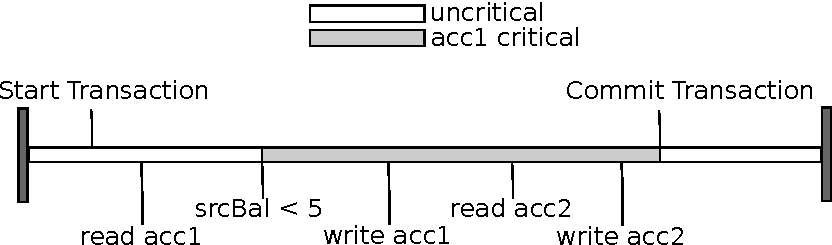
\includegraphics{Figures/lessCriticalValue}
\decoRule
\caption[lessCriticalValue]{The critical time of \code{limmitedTransfer} with the alternative implementation.}
\label{fig:lessCriticalValue}
\end{figure}
The TVar \code{acc2} is not critical at any point in the transaction, because it is not needed for the control 
flow. \code{acc1} on the other hand becomes critical at the time its value is used to evaluate the branch
condition \code{(srcBal < am)}.


When the commit phase
begins the transaction is validated. The validation does not differ from the validation in the original implementation.
When a \code{readTVar} is evaluated the current value of the TVar is logged. Validating the transactions means to 
check if the values logged match the actual values of the TVars. If the transaction is not valid it is rolled back.
If the transaction is valid, the TVars it has accessed are locked and the remaining \code{readtVar} operations are
evaluated. At this point no other transaction is able to modify the TVars and thus the evaluation is safe in the sense
that the value cannot change until the commit of the transaction is completed. After the reads are evaluated the 
writes are processed and the result is returned after unlocking the TVars.

%TODO example


